

\myNewSlide
\large
\begin{picture}(500,0)(0,0)
      \put(-200,-190){\makebox(0,0)[l]{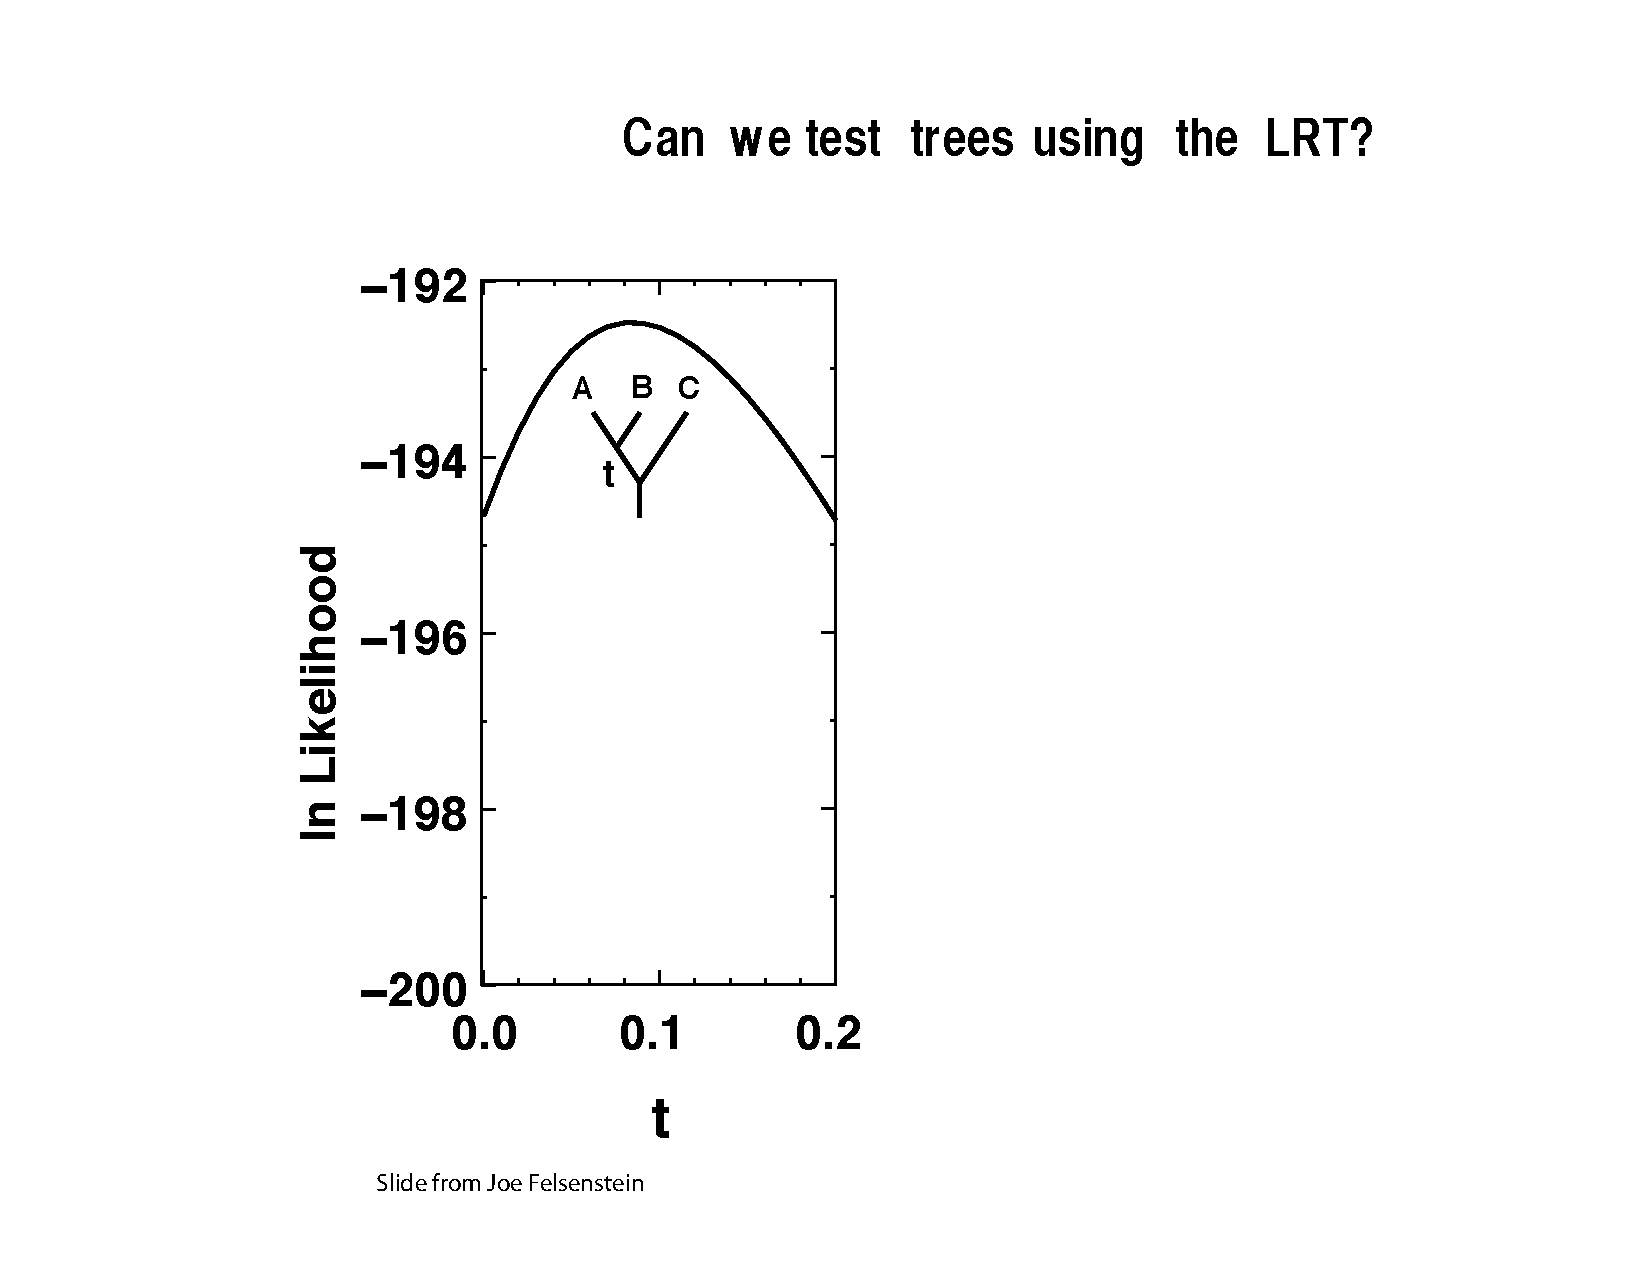
\includegraphics[scale=1.0]{../newimages/JoeFelsTreeLRT1.pdf}}}
      \put(250,-100){1. Should we calculate the LRT as:}
      \put(224,-140){$\delta_i = 2\left[\ln L(t=\hat{t},T_i \mid X) - \ln L(t=0,T_i \mid X)\right]$}
      \put(250,-250){2. And can we use the $\chi_1^2$ distribution to}
      \put(250,-290){get the critical value for $\delta$?}
\end{picture}

\myNewSlide
\begin{picture}(500,0)(0,0)
      \put(-200,-190){\makebox(0,0)[l]{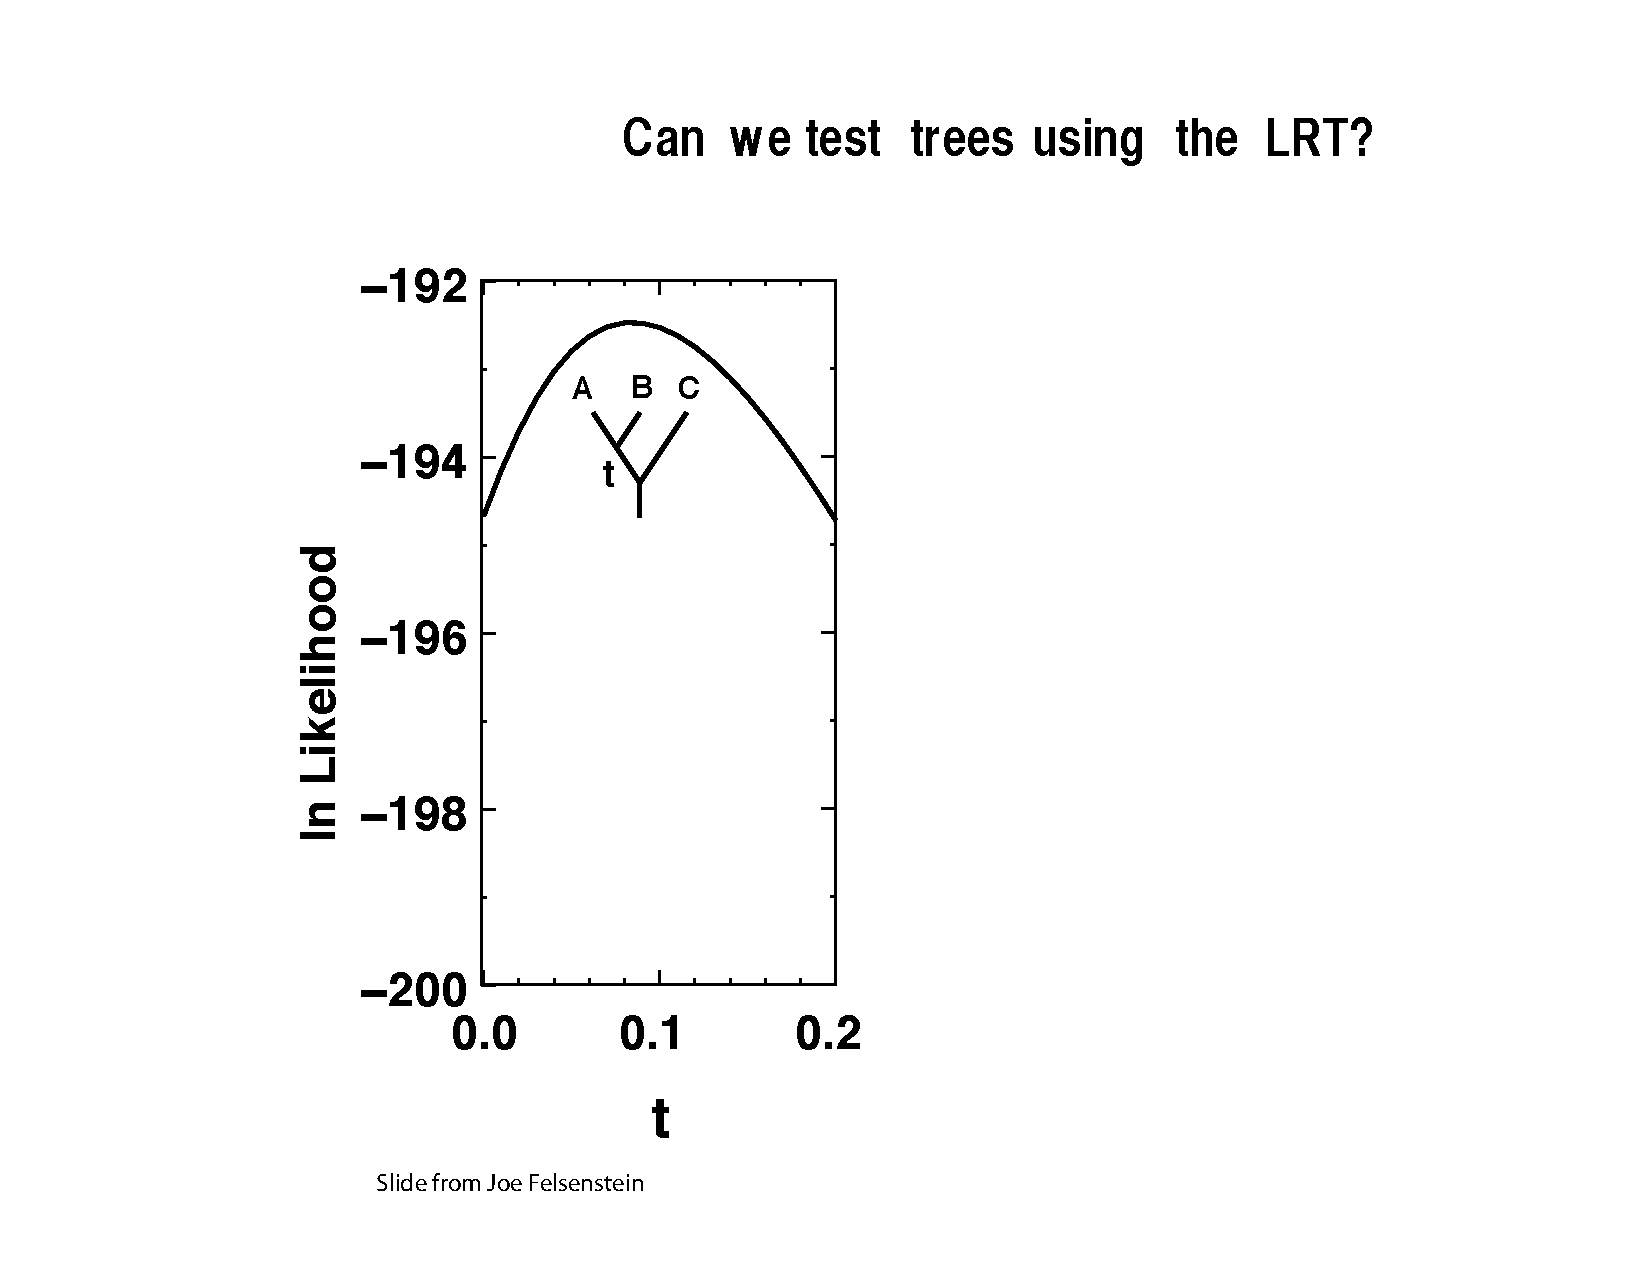
\includegraphics[scale=1.0]{../newimages/JoeFelsTreeLRT1.pdf}}}
      \put(250,-100){1. Should we calculate the LRT as:}
      \put(224,-140){$\delta_i = 2\left[\ln L(t=\hat{t},T_i \mid X) - \ln L(t=0,T_i \mid X)\right]$}
      \put(250,-180){{\bf \color{red}No. $t=0$ might not yield the best}}
      \put(260,-220){\bf\color{red} alternative $\ln L$}
      \put(250,-290){2. And can we use the $\chi_1^2$ distribution to}
      \put(250,-330){get the critical value for $\delta$ ?}
      \put(250,-370){{\bf \color{red}No. Constraining parameters}}
      \put(260,-410){{\bf \color{red}at boundaries leads to a mixture}}
      \put(260,-450){{\bf \color{red}such as: $\frac{1}{2}\chi_0^2 + \frac{1}{2}\chi_1^2$}}
      \put(260,-490){\small See \citet{OtaWHSK2000}.}
\end{picture}

\myNewSlide
\section*{aLRT of \citet{AnisimovaG2006}}
\begin{compactitem}
    \item For a {\bf branch} $j$, calculate $\delta_{j}^{\dag}$ as twice the difference in $\ln L$ between the optimal tree (which has the branch) and the best NNI neighbor.
    \item This is very fast.
    \item They argue that the null distribution for each LRT around the polytomy follows a $\frac{1}{2}\chi_0^2 + \frac{1}{2}\chi_1^2$ distribution
    \item The introduce Bonferroni-correction appropriate for correcting for the selection of the best of the three resolutions.
    \item They find aLRT to be accurate and powerful in simulations, but \citet{AnisimovaGDDG2011} report that it rejects too often and is sensitive to model violation.
\end{compactitem}

\myNewSlide
\begin{picture}(500,0)(0,0)
      \put(-130,-450){\makebox(0,0)[l]{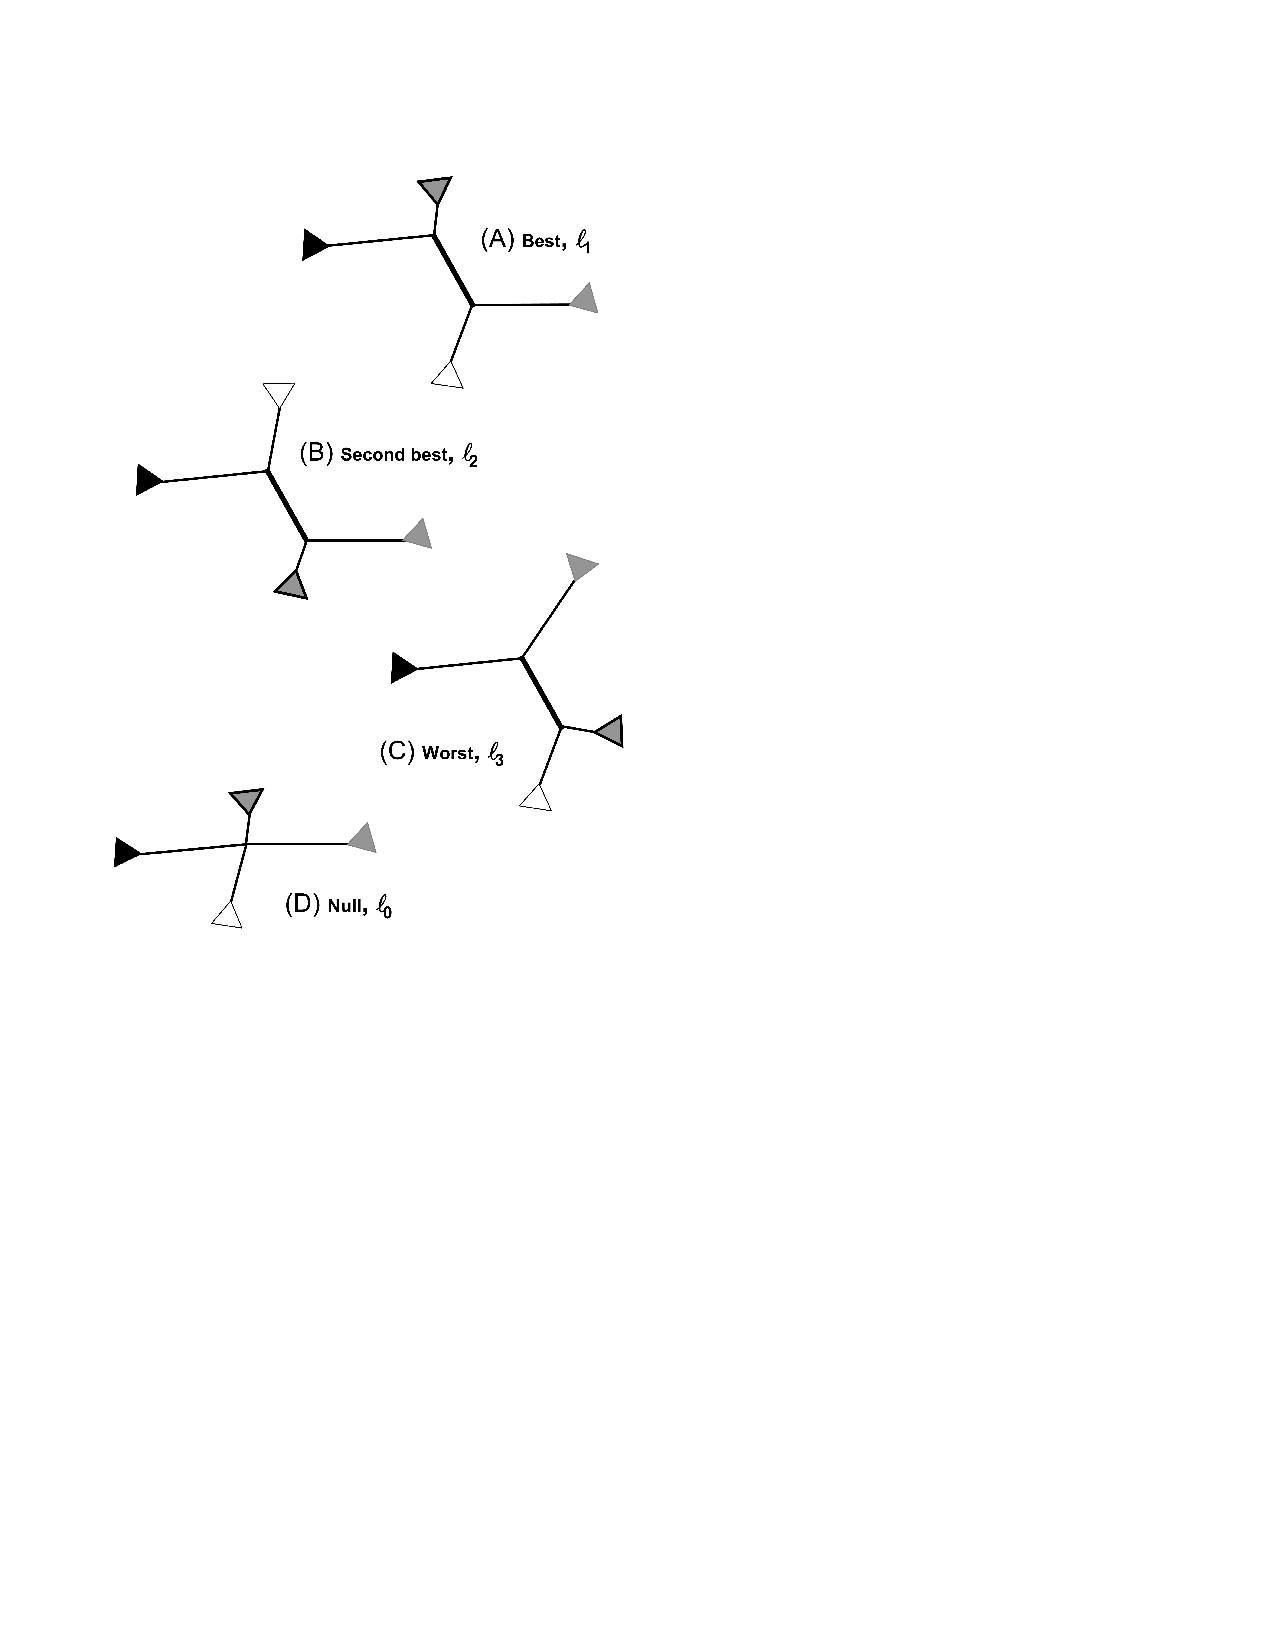
\includegraphics[scale=1.5]{../newimages/AnisimovaG2006Fig1.pdf}}}
      \put(300,-200){aLRT = $2\left[\ln \ell_1 - \ln L(T_2 \mid X)\right]$}
      \put(300,-240){$\ell_1 = L(T_1 \mid X)$}
      \put(400,-400){\small Image from \citet{AnisimovaG2006}}
\end{picture}

\myNewSlide
\section*{aBayes \citet{AnisimovaGDDG2011} }


$$\mbox{aBayes}(T_1 \mid X) = \frac{\Pr(X \mid T_1)}{\Pr(X \mid T_1) + \Pr(X \mid T_2) + \Pr(X \mid T_3)}$$

Simulation studies of \citet{AnisimovaGDDG2011} show it to have the best power of the methods that do not have inflated probability of falsely rejecting the null.

It is sensitive to model violation.

This is similar to ``likelihood-mapping'' of \citet{StrimmerVH1997}


\myNewSlide
\begin{picture}(500,0)(0,0)
      \put(-200,-190){\makebox(0,0)[l]{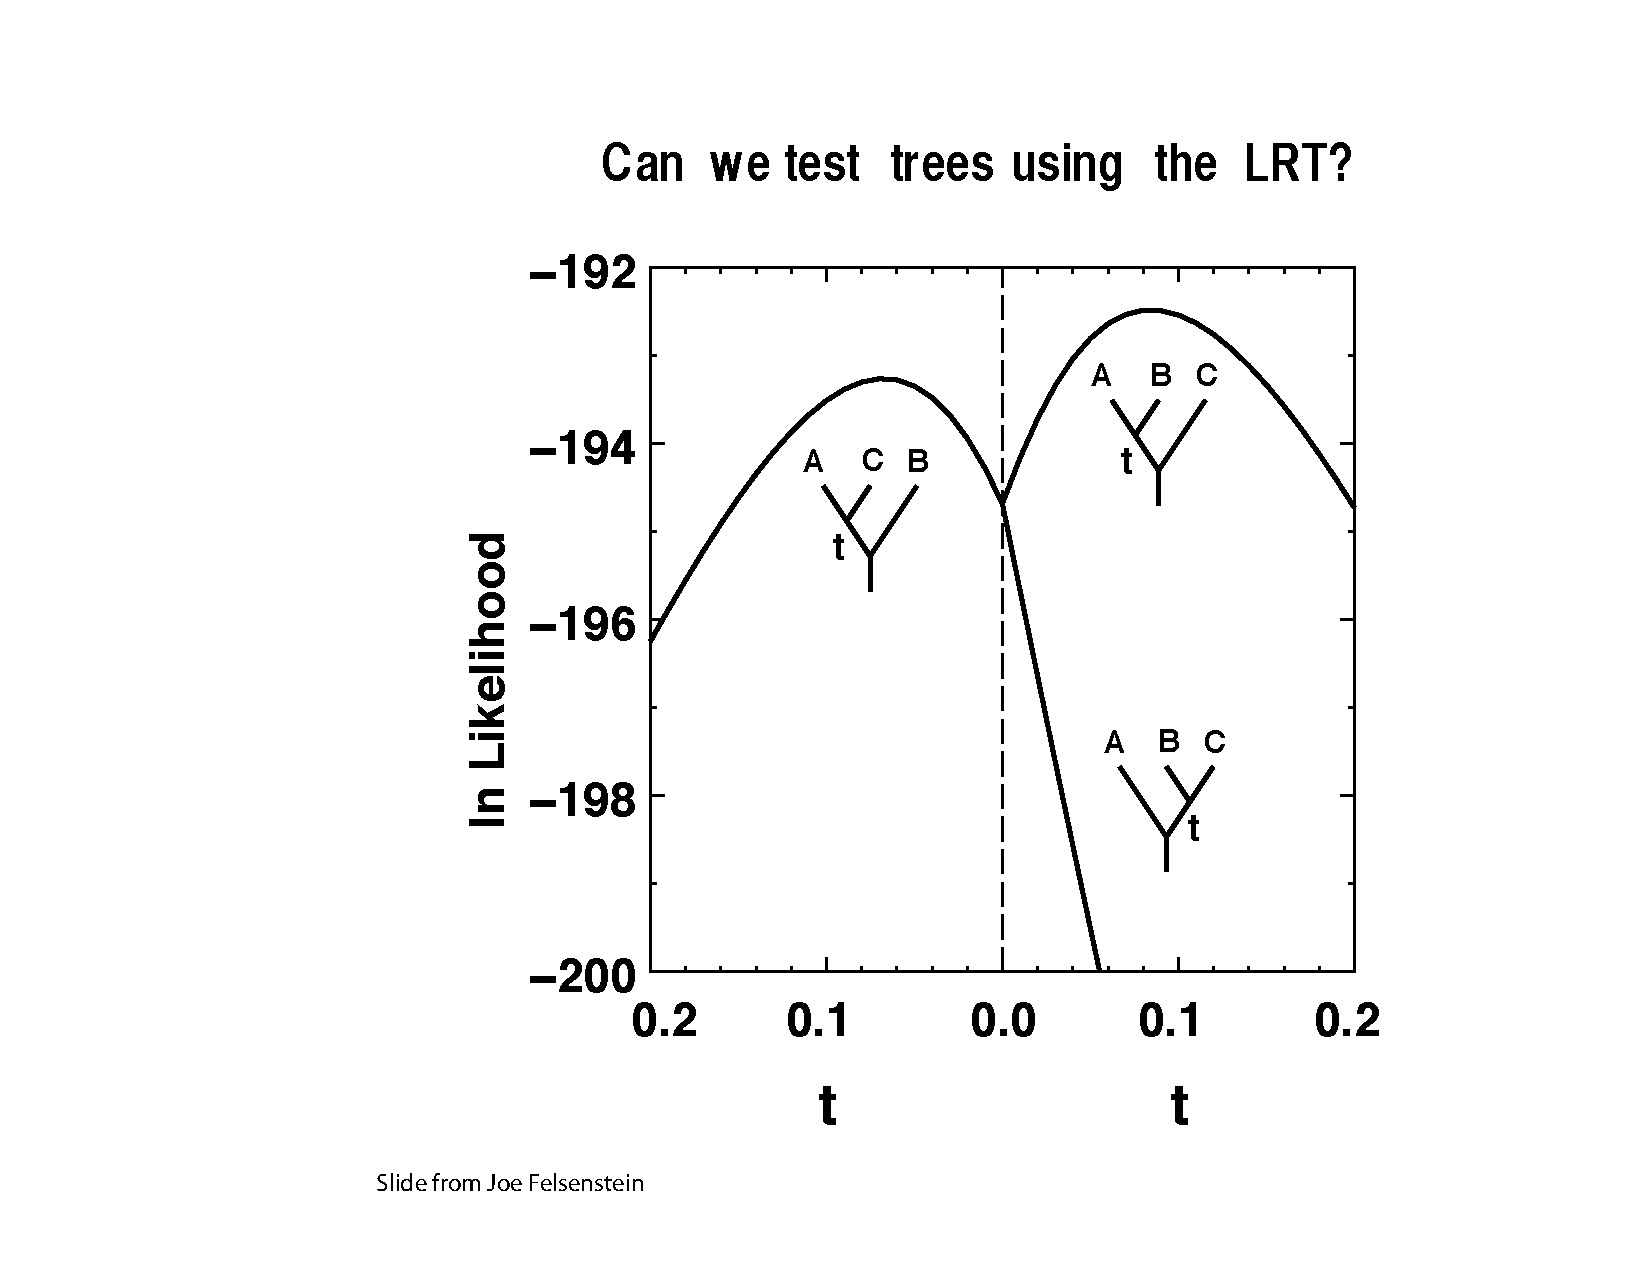
\includegraphics[scale=1.0]{../newimages/JoeFelsTreeLRT2.pdf}}}
      \put(470,-170){{\bf \color{red}No, tree hypotheses}}
      \put(470,-200){{\bf \color{red}are not nested! }}
\end{picture}


\myNewSlide
\section*{coin flipping example (again, for inspiration)}
$N=100$ and $H=60$

Can we reject the hypothesis of a fair coin?

We can use simulation to generate the null distribution (we could actually use the binomial distribution to analytically solve this one)...


\myNewSlide
\begin{picture}(0,0)(0,0)
    \put(-10,-250){\makebox(0,0)[l]{\includegraphics[scale=1.0]{/home/mtholder/Documents/ku_teaching/BIOL-848-2013/images/nullhist.pdf}}}
    \put(150,-250){\color{red} P-value $\approx$ 0.029 }
\end{picture}

\myNewSlide
\section*{The simplest phylogenetic test would compare two trees}
\Large
Null: If we had no sampling error (infinite data) $T_1$ and $T_2$ would explain the data equally well. 

Test Statistic: $$\delta(T_1,T_2 \mid X) = 2\left[\ln L(T_1 \mid X) - \ln L(T_2 \mid X)\right]$$

Expectation under null: $$\mathbb{E}_{H_0}\left[\delta(T_1,T_2 \mid X)\right] = 0$$


\myNewSlide
\begin{picture}(500,0)(-20,-50)
      \put(20,-20){\small Using 3000 sites of mtDNA sequence for 5 primates}
      \put(20,-60){\normalsize $T_1$ is ((chimp, gorilla), human)}
      \put(50,-200){\makebox(0,-190)[l]{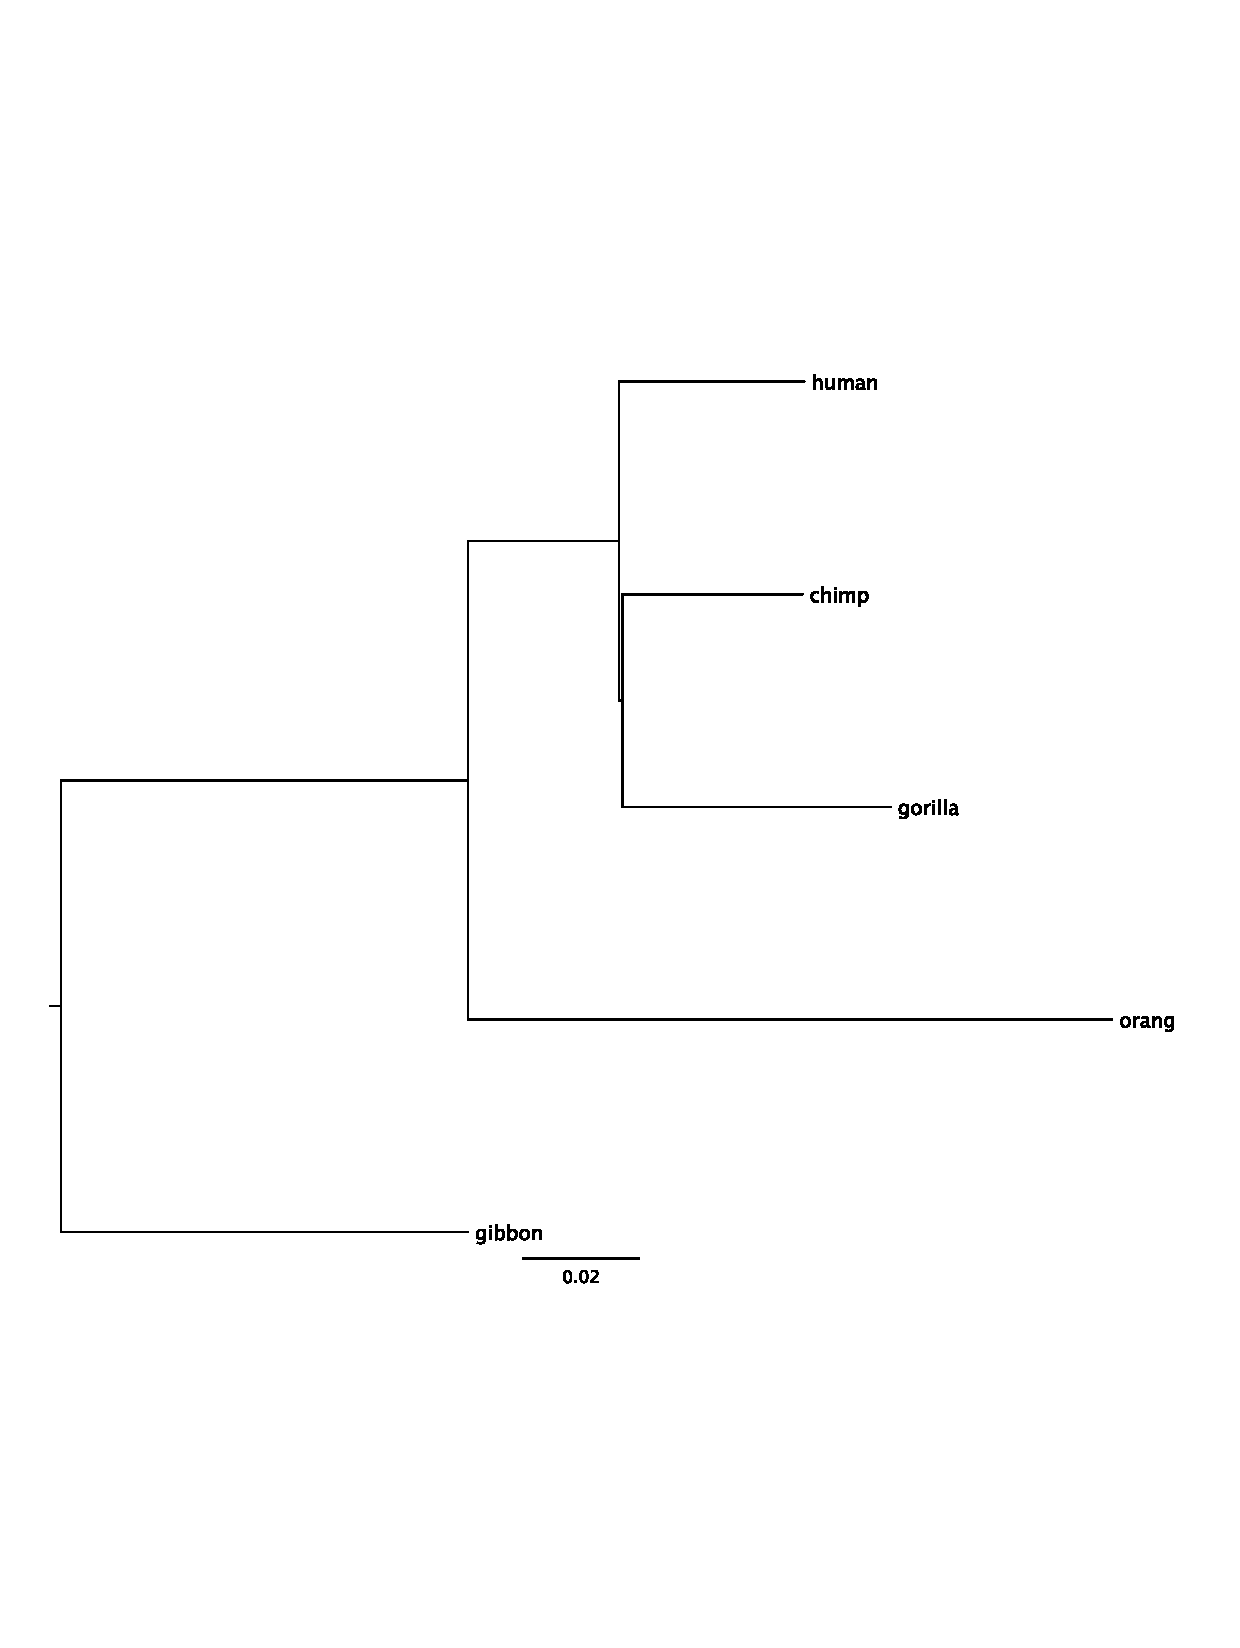
\includegraphics[scale=1.0]{../scripts/mtdna/chimpGorilla3000sites.pdf}}}
\end{picture}

\myNewSlide
\begin{picture}(500,0)(-20,-50)
      \put(20,-20){\small Using 3000 sites of mtDNA sequence for 5 primates}
      \put(20,-60){\normalsize $T_2$ is ((chimp, human), gorilla)}
      \put(50,-200){\makebox(0,-190)[l]{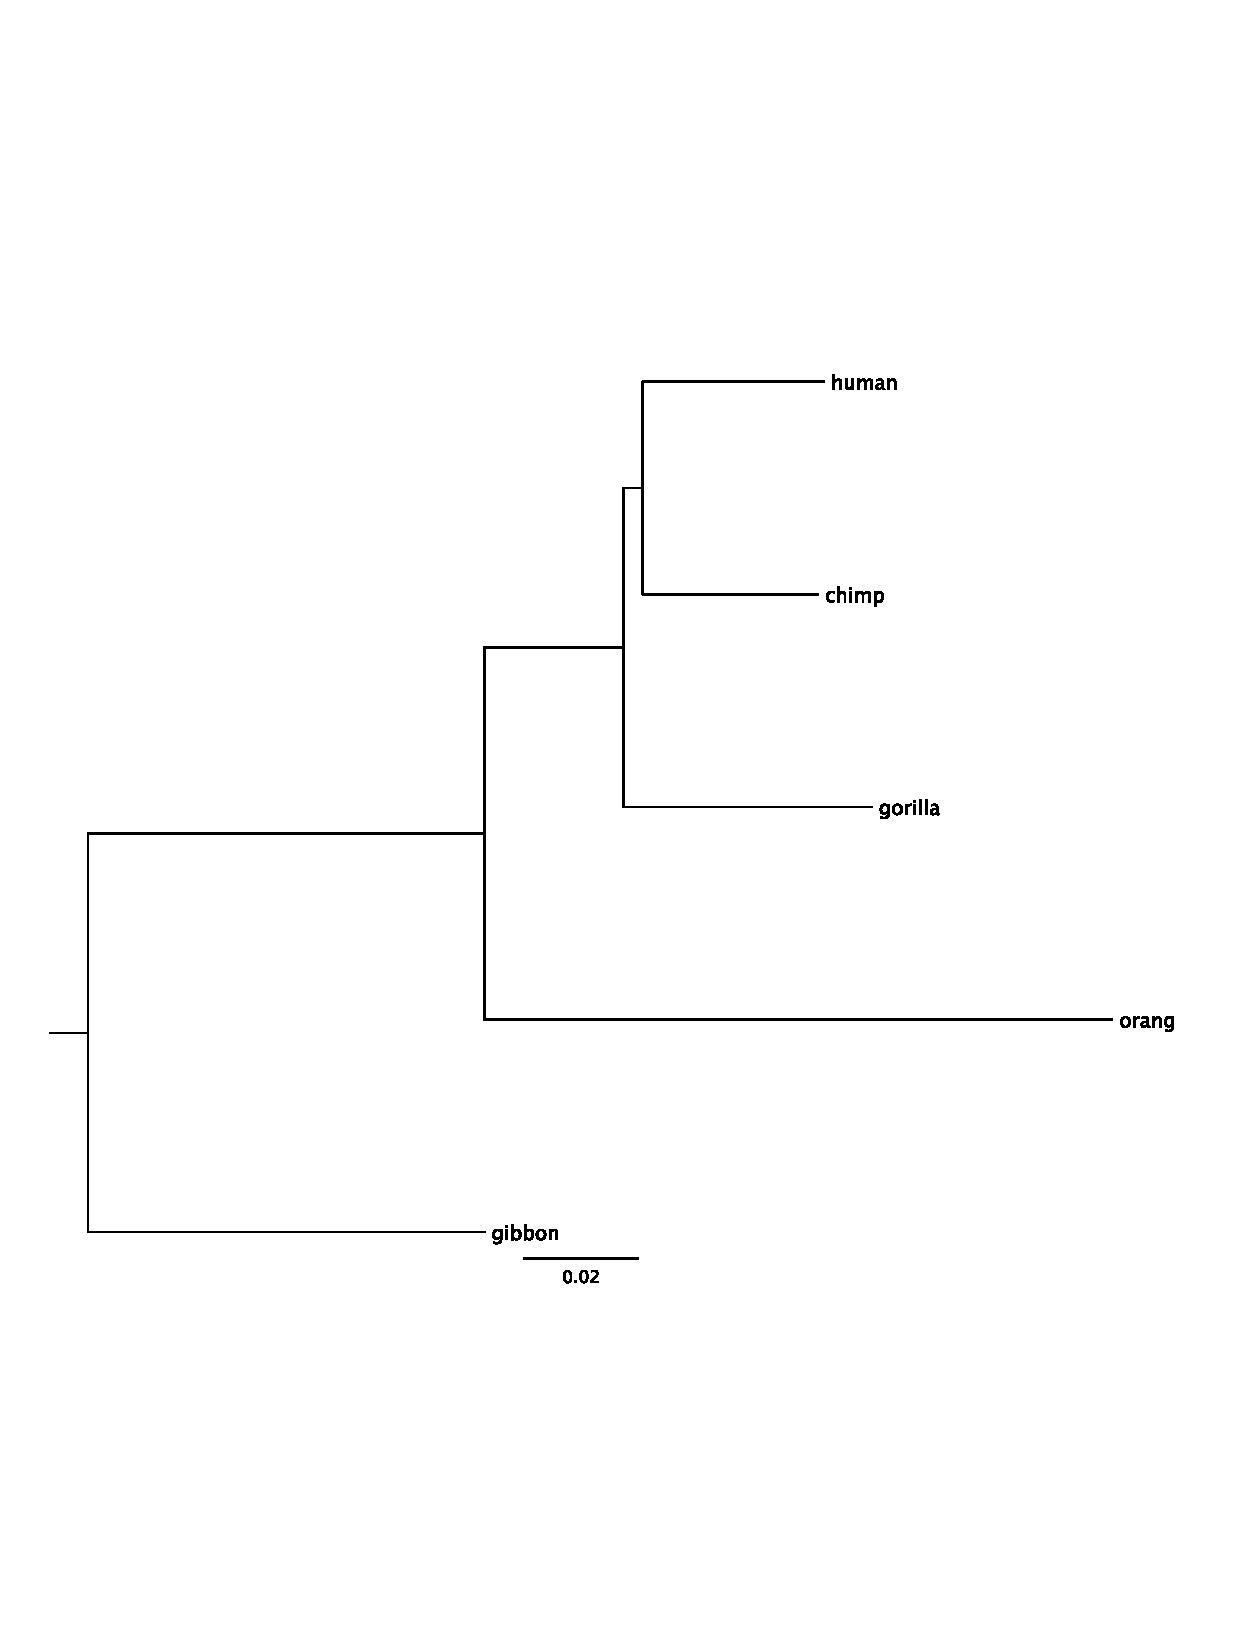
\includegraphics[scale=1.0]{../scripts/mtdna/humanChimp3000SitesTree.pdf}}}
\end{picture}

\myNewSlide
\begin{picture}(500,0)(-20,-50)
      \put(20,-20){\small Using 3000 sites of mtDNA sequence for 5 primates}
      \put(20,-60){\normalsize $T_1$ is ((chimp, gorilla), human)   \hskip2cm $\ln L(T_1 \mid X) = -7363.296$}
      \put(20,-100){\normalsize $T_2$ is ((chimp, human), gorilla)  \hskip2cm $\ln L(T_2 \mid X) = -7361.707$}
      \put(-10,-385){\small$\delta(T_1,T_2 \mid X)=-3.18$}
      \put(300,-385){\small$\mathbb{E}(\delta)$}
      \put(50,-150){\makebox(0,-190)[l]{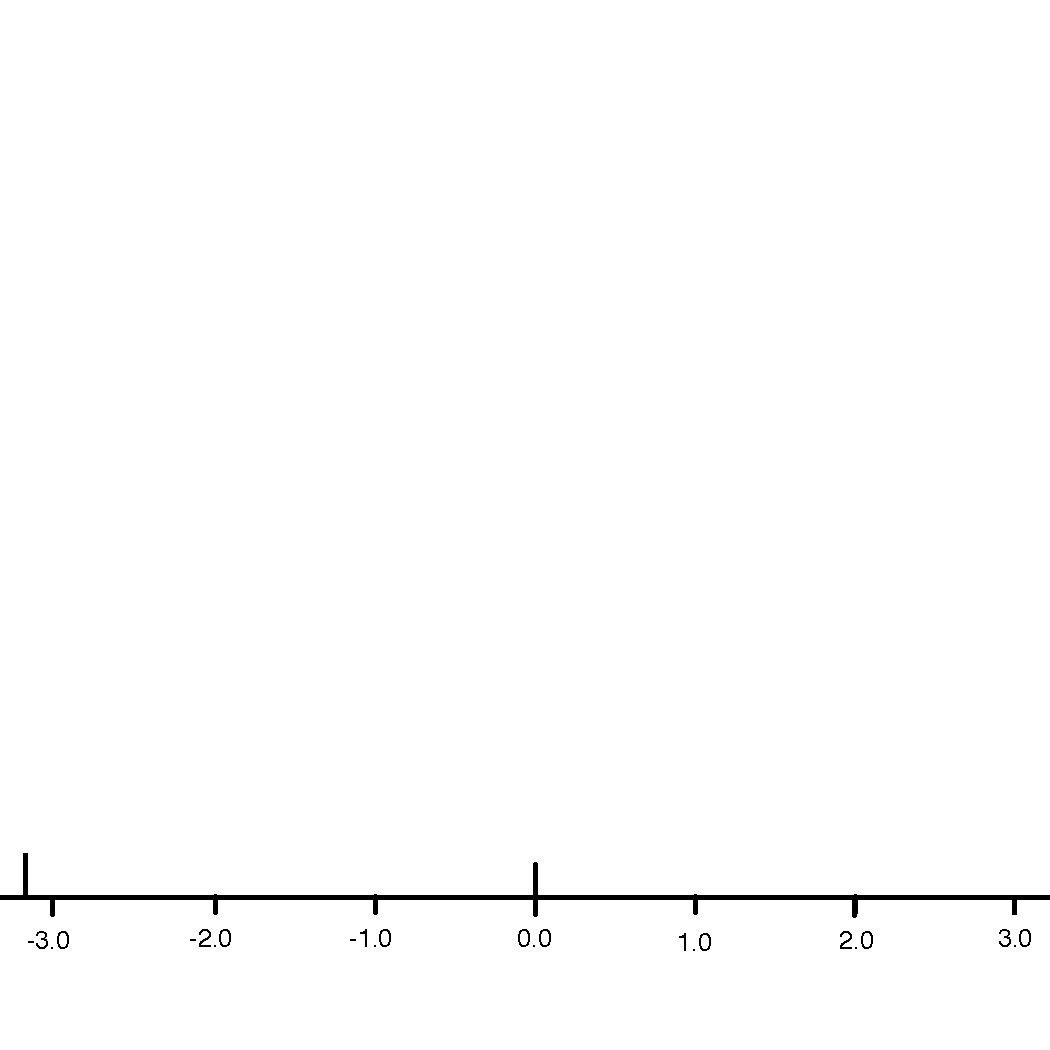
\includegraphics[scale=1.0]{../newimages/delta_axes.pdf}}}
      \put(220,-480){$\delta(T_1,T_2 \mid X) $}
\end{picture}




\myNewSlide

To get the $P$-value, we need to know the probability: $$\Pr\left(\big | \delta(T_1,T_2 \mid X)\big |  \geq 3.18  {\bm{\Big|}}  H_0\mbox{ is true}\right) $$
\begin{picture}(500,0)(-20,-50)
      \put(-10,-235){\small$\delta(T_1,T_2 \mid X)=-3.18$}
      \put(460,-235){\small$-\delta(T_1,T_2 \mid X)=3.18$}
      \put(10,-270){\huge$\leftarrow$}
      \put(570,-270){\huge$\rightarrow$}
      \put(300,-235){\small$\mathbb{E}(\delta)$}
      \put(50,-0){\makebox(0,-190)[l]{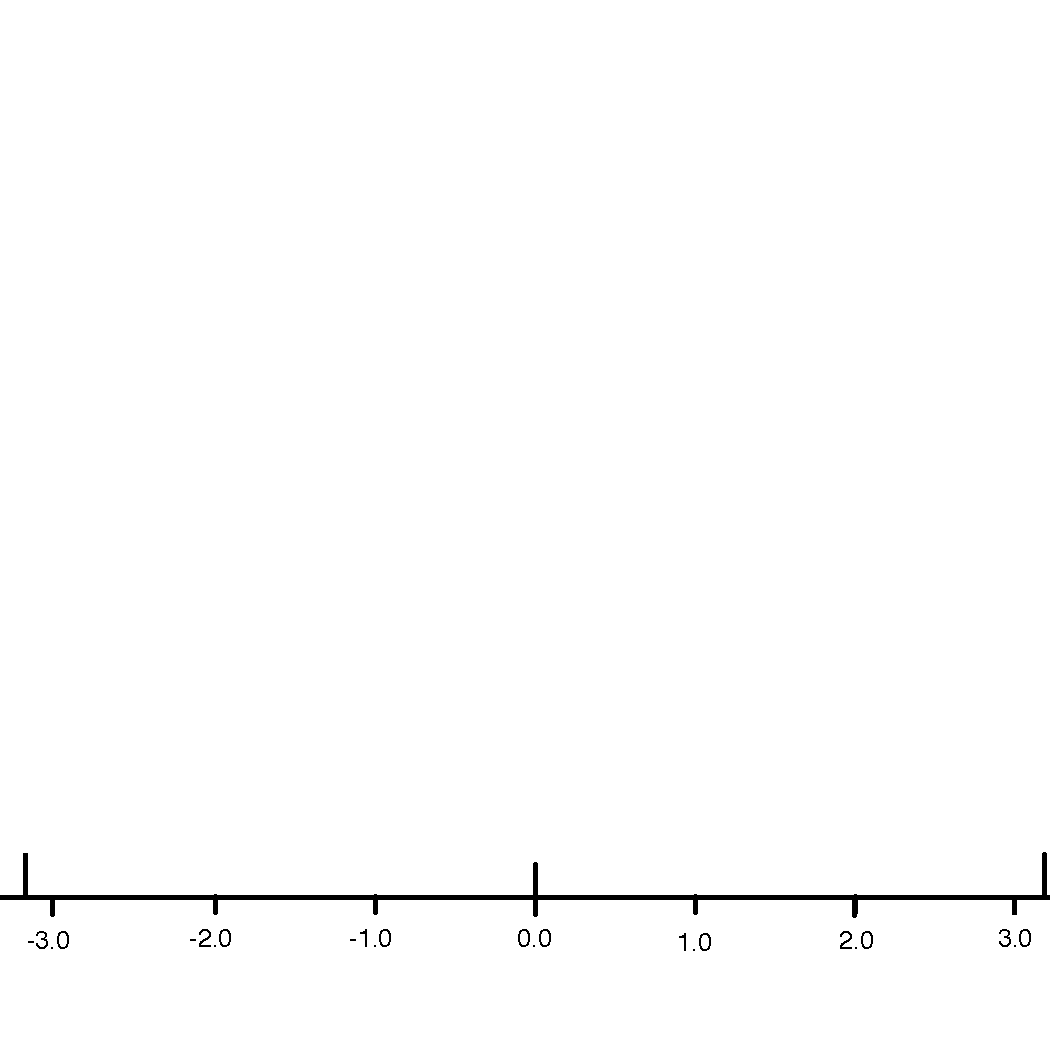
\includegraphics[scale=1.0]{../newimages/delta_axes_reflected.pdf}}}
      \put(220,-330){$\delta(T_1,T_2 \mid X) $}
\end{picture}

\myNewSlide
\section*{KH Test}
\begin{compactenum}
    \item Examine the difference in $\ln L$ for each site: $\delta(T_1,T_2 \mid X_i)$ for site $i$.
    \item Note that the total difference is simply a sum:
        $$\delta(T_1,T_2 \mid X) = \sum_{i=1}^M\delta(T_1,T_2 \mid X_i)$$
    \item The variance of $\delta(T_1,T_2 \mid X)$ will be a function of the variance in ``site'' $\delta(T_1,T_2 \mid X_i)$ values.
\end{compactenum}



\myNewSlide
\begin{picture}(500,0)(0,0)
      \put(0,10){\large $\delta(T_1,T_2 \mid X_i)$ for each site, $i$.}
      \put(280,-35){\large $\vdots$}
      \put(20,-250){\makebox(0,0)[l]{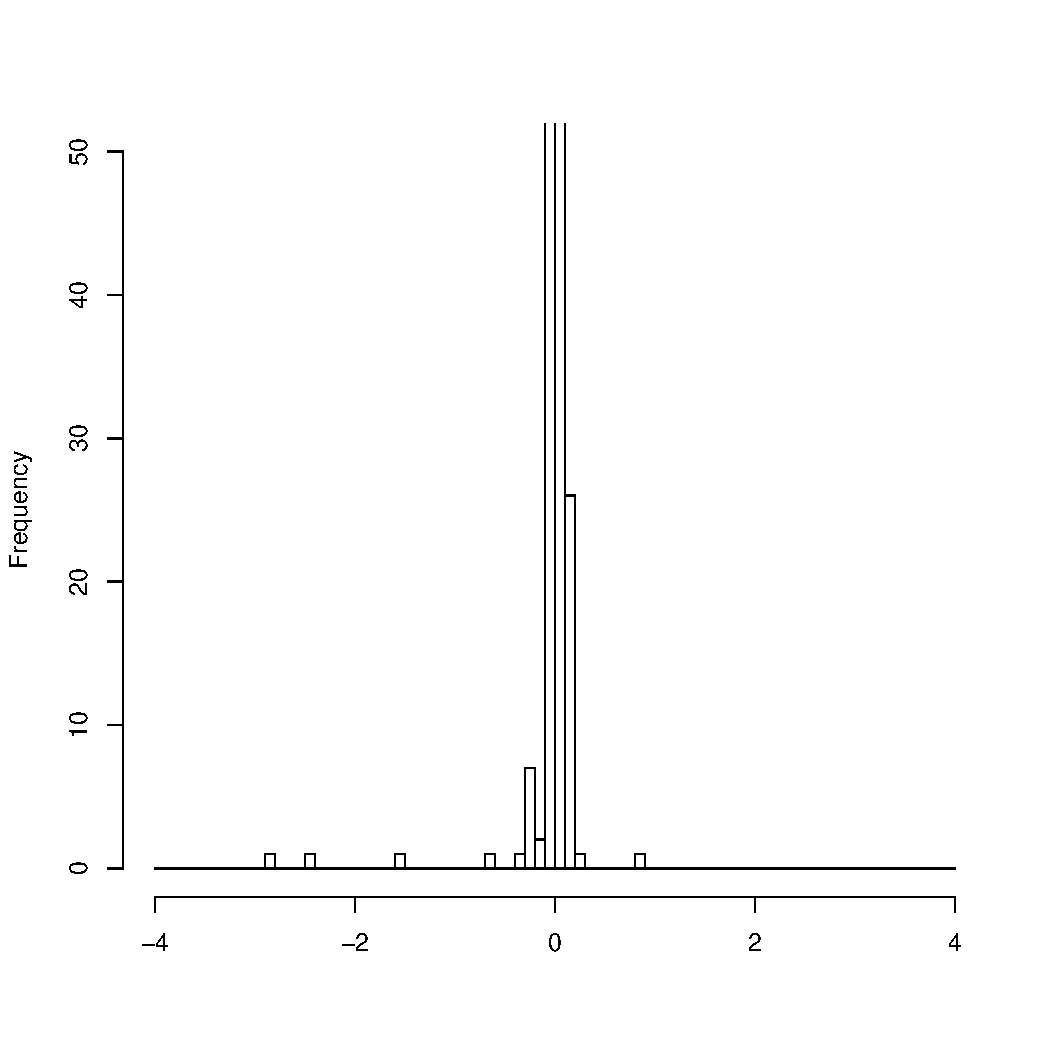
\includegraphics[scale=1.0]{../scripts/mtdna/d1-2hist.pdf}}}
      \put(250,-490){\normalsize$\delta(T_1,T_2 \mid x_i)$}
\end{picture}


\myNewSlide
\section*{KH Test - the variance of $\delta(T_1,T_2 \mid X)$}
To approximate variance of $\delta(T_1,T_2 \mid X)$ under the null, we could:
\begin{compactenum}
    \item use assumptions of Normality (by appealing to the Central Limit Theorem\footnote{\citet{Susko2014} recently showed that this is flawed and too conservative.}). Or
    \item use bootstrapping to generate a cloud of pseudo-replicate $\delta(T_1,T_2 \mid X^{\ast})$ values, and look at their variance.
\end{compactenum}

\myNewSlide
\begin{picture}(500,0)(0,0)
      \put(0,-10){\large $\delta$ for many (RELL) bootstrapped replicates of the data}
      \put(20,-250){\makebox(0,0)[l]{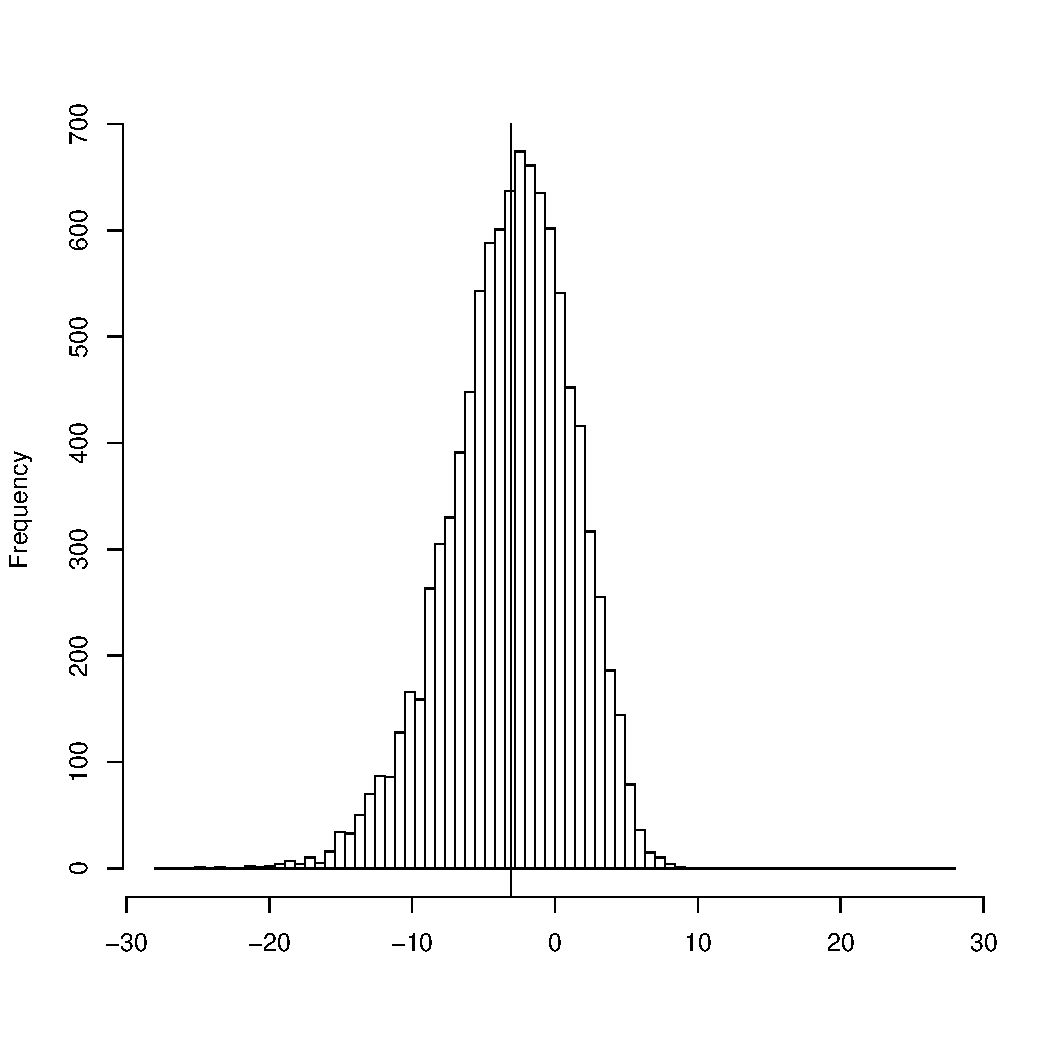
\includegraphics[scale=1.0]{../scripts/mtdna/uncentered1-2hist.pdf}}}
      \put(250,-490){\normalsize$\delta(T_1,T_2 \mid X^{\ast})$}
\end{picture}



\myNewSlide
\begin{picture}(500,0)(0,0)
      \put(0,10){\large The (RELL) bootstrapped sample of statistics.}
      \put(0,-20){\large Is this the null distribution for our $\delta$ test statistic?}
      \put(20,-250){\makebox(0,0)[l]{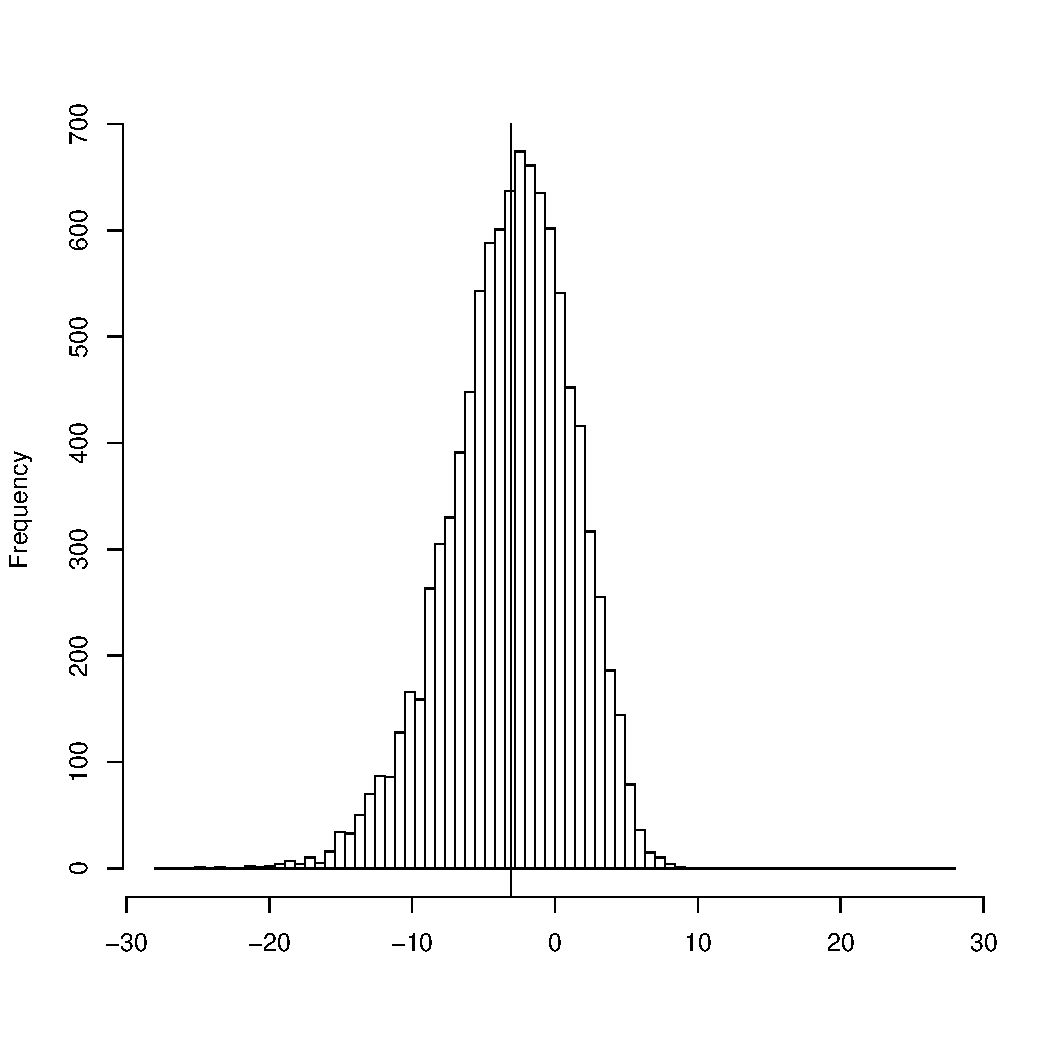
\includegraphics[scale=1.0]{../scripts/mtdna/uncentered1-2hist.pdf}}}
      \put(250,-490){\normalsize$\delta(T_1,T_2 \mid X^{\ast})$}
\end{picture}

\myNewSlide
\section*{KH Test - `centering'}
{\begin{center} $\mathbb{E}_{H_0}\left[\delta(T_1,T_2 \mid X)\right] = 0$\end{center}}\\
Bootstrapping gives us a reasonable guess of the variance under $H_0$

Subtracting the mean of the bootstrapped $\delta(T_1,T_2 \mid X^{\ast})$ values gives the null distribution.

For each of the $j$ bootstrap replicates, we treat $$\delta(T_1,T_2 \mid X^{\ast j}) - \bar\delta(T_1,T_2 \mid X^{\ast})$$  as draws from the null distribution.

\myNewSlide
\begin{picture}(500,0)(0,0)
      \put(0,10){\large $\delta(T_1,T_2 \mid X^{(j)})-\bar\delta(T_1,T_2 \mid X^{\ast})$}
      \put(0,-25){for many (RELL) bootstrapped replicates of the data}
      \put(20,-250){\makebox(0,0)[l]{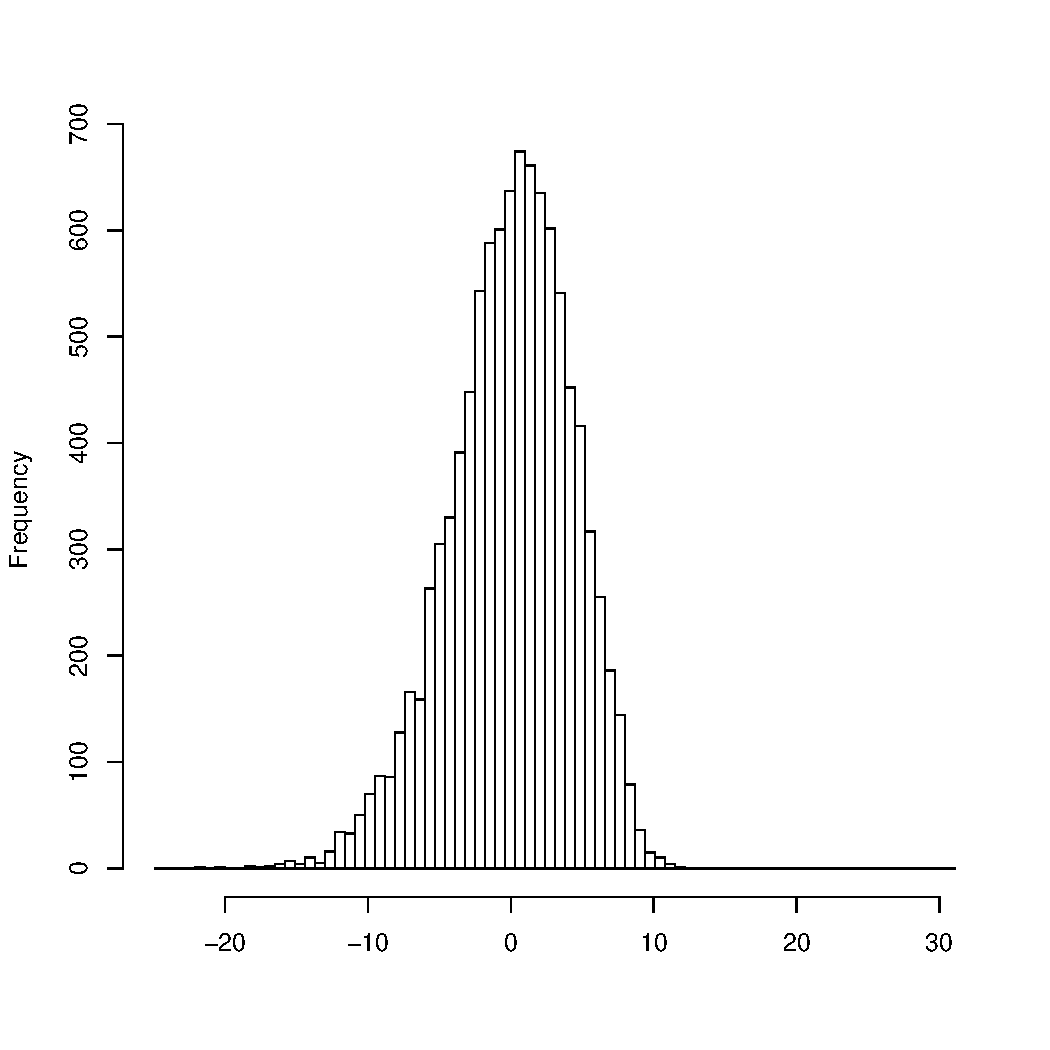
\includegraphics[scale=1.0]{../scripts/mtdna/centered1-2hist.pdf}}}
      \put(150,-490){\normalsize$\delta(T_1,T_2 \mid X^{(j)})-\bar\delta(T_1,T_2 \mid X^{\ast})$}
\end{picture}

\myNewSlide
\begin{picture}(500,0)(0,0)
      \put(0,10){Approximate null distribution with}
      \put(0,-30){tails (absolute value $\geq 3.18$) shown}
      \put(20,-250){\makebox(0,0)[l]{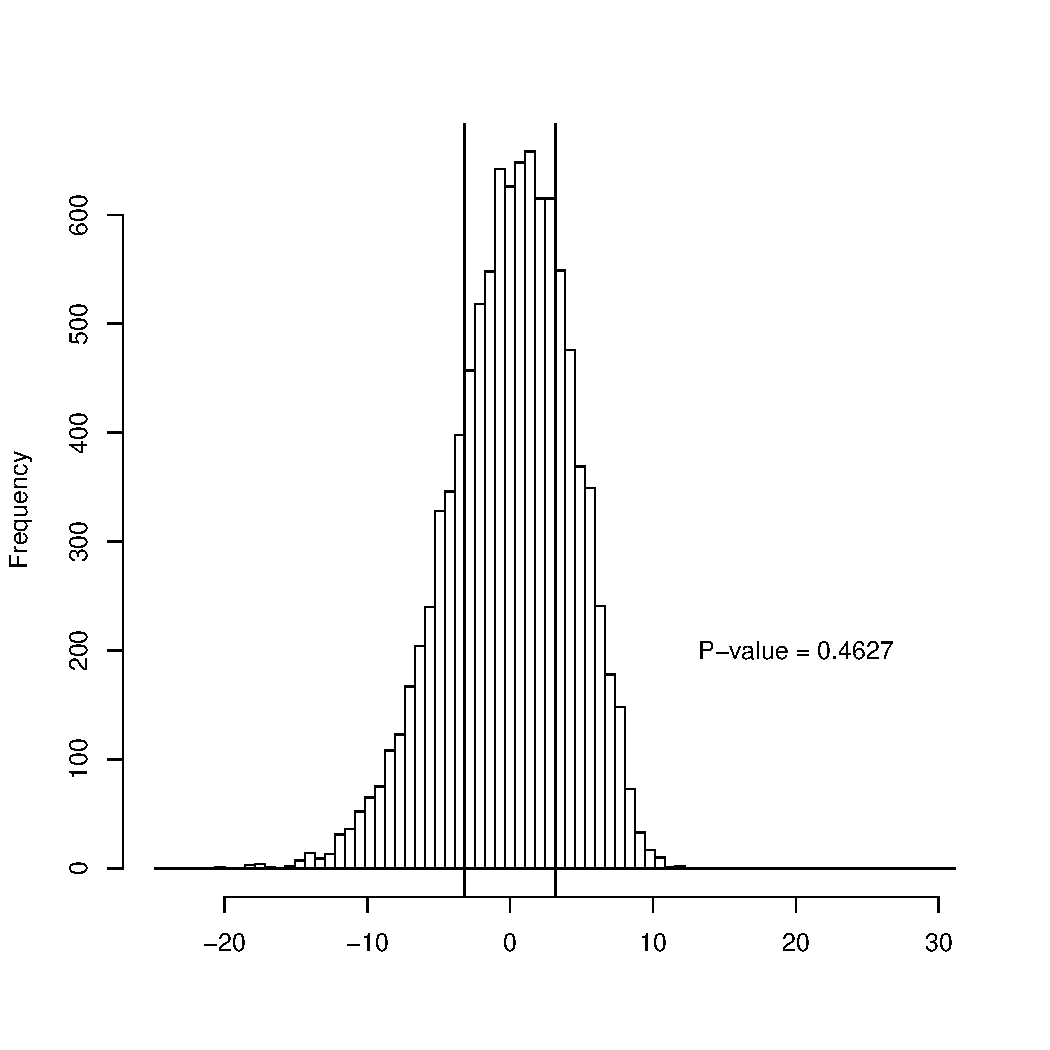
\includegraphics[scale=1.0]{../scripts/mtdna/centered1-2hist-p.pdf}}}
      \put(175,-490){\normalsize$\delta(T_1,T_2 \mid X^{\ast})-\bar\delta(T_1,T_2 \mid X^{\ast})$}
\end{picture}




\myNewSlide
\section*{Other ways to assess the null distribution of the LR test statistic}
\begin{itemize}
    \item Bootstrapping then centering LR, and 
    \item Using normality assumptions.
\end{itemize}
are both clever and cute solutions.

They are too conservative \citep{Susko2014} - more complicated calculations from the Normal [KHns] or mixtures of $\chi^2$ distributions [chi-bar].

They do not match the null distribution under any model of sequence evolution.


\myNewSlide
\section*{Mini-summary}

\begin{itemize}
    \item $\delta(T_1,T_2 \mid X) = 2\left[\ln L(T_1 \mid X) - \ln L(T_2 \mid X)\right]$ is a powerful statistic for discrimination between trees.
    \item We can assess confidence by considering the variance in signal between different characters.
    \item Bootstrapping helps us assess the variance in $\ln L$ that we would expect to result from sampling error.
\end{itemize}


